%%%%%%%%%%%%%%%%%%%%%%%%%%%%%%%%%%%%%%%%%
% Beamer Presentation
% LaTeX Template
% Version 1.0 (10/11/12)
%
% This template has been downloaded from:
% http://www.LaTeXTemplates.com
%
% License:
% CC BY-NC-SA 3.0 (http://creativecommons.org/licenses/by-nc-sa/3.0/)
%
%%%%%%%%%%%%%%%%%%%%%%%%%%%%%%%%%%%%%%%%%

%----------------------------------------------------------------------------------------
%	PACKAGES AND THEMES
%----------------------------------------------------------------------------------------

\documentclass{beamer}

\mode<presentation> {

%\usetheme{default}
%\usetheme{AnnArbor}
%\usetheme{Antibes}
%\usetheme{Bergen}
%\usetheme{Berkeley}
%\usetheme{Berlin}
%\usetheme{Boadilla}
%\usetheme{CambridgeUS}
%\usetheme{Copenhagen}
%\usetheme{Darmstadt}
%\usetheme{Dresden}
\usetheme{Frankfurt}
%\usetheme{Goettingen}
%\usetheme{Hannover}
%\usetheme{Ilmenau}
%\usetheme{JuanLesPins}
%\usetheme{Luebeck}
%\usetheme{Madrid}
%\usetheme{Malmoe}
%\usetheme{Marburg}
%\usetheme{Montpellier}
%\usetheme{PaloAlto}
%\usetheme{Pittsburgh}
%\usetheme{Rochester}
%\usetheme{Singapore}
%\usetheme{Szeged}
%\usetheme{Warsaw}

%\usecolortheme{albatross}
%\usecolortheme{beaver}
%\usecolortheme{beetle}
%\usecolortheme{crane}
%\usecolortheme{dolphin}
%\usecolortheme{dove}
%\usecolortheme{fly}
%\usecolortheme{lily}
%\usecolortheme{orchid}
%\usecolortheme{rose}
%\usecolortheme{seagull}
%\usecolortheme{seahorse}
%\usecolortheme{whale}
%\usecolortheme{wolverine}

%\setbeamertemplate{footline} % To remove the footer line in all slides uncomment this line
%\setbeamertemplate{footline}[page number] % To replace the footer line in all slides with a simple slide count uncomment this line

%\setbeamertemplate{navigation symbols}{} % To remove the navigation symbols from the bottom of all slides uncomment this line
}

\usepackage{graphicx} % Allows including images
\usepackage{booktabs} % Allows the use of \toprule, \midrule and \bottomrule in tables
\usepackage[spanish]{babel}
\usepackage[utf8]{inputenc}
\usepackage[T1]{fontenc}
\usepackage{textcomp}
\usepackage{geometry}
%\usepackage{movie15}
\usepackage{hyperref}

%----------------------------------------------------------------------------------------
%	TITLE PAGE
%----------------------------------------------------------------------------------------

\title[LZW CoDec]{LZW Compressor and Decompressor Algorithm} % The short title appears at the bottom of every slide, the full title is only on the title page

\author{Javier Acosta\\Daniel Méndez\\Willy Villalobos} % Your name
\institute[UCR] % Your institution as it will appear on the bottom of every slide, may be shorthand to save space
{
Universidad de Costa Rica \\ % Your institution for the title page
\medskip
\textit{} % Your email address
}
\date{\today} % Date, can be changed to a custom date

\begin{document}

	\begin{frame}
		\titlepage % Print the title page as the first slide
	\end{frame}

%\begin{frame}
%\frametitle{Overview} % Table of contents slide, comment this block out to remove it
%\tableofcontents % Throughout your presentation, if you choose to use \section{} and \subsection{} commands, these will automatically be printed on this slide as an overview of your presentation
%\end{frame}

%----------------------------------------------------------------------------------------
%	PRESENTATION SLIDES
%----------------------------------------------------------------------------------------

%------------------------------------------------
%\section{First Section} % Sections can be created in order to organize your presentation into discrete blocks, all sections and subsections are automatically printed in the table of contents as an overview of the talk
%------------------------------------------------

%\subsection{Subsection Example} % A subsection can be created just before a set of slides with a common theme to further break down your presentation into chunks

%----------------------------------------------------------------------------------------
%----------------------------------------------------------------------------------------

	\begin{frame}
		\frametitle{¿Qué es LZW?}
		Es un algoritmo de compresión sin pérdida desarrollado en 1984 por Terry Welch. La actual implementación hace uso de la función hash para comprimir y descomprimir los datos.

		\begin{figure}
			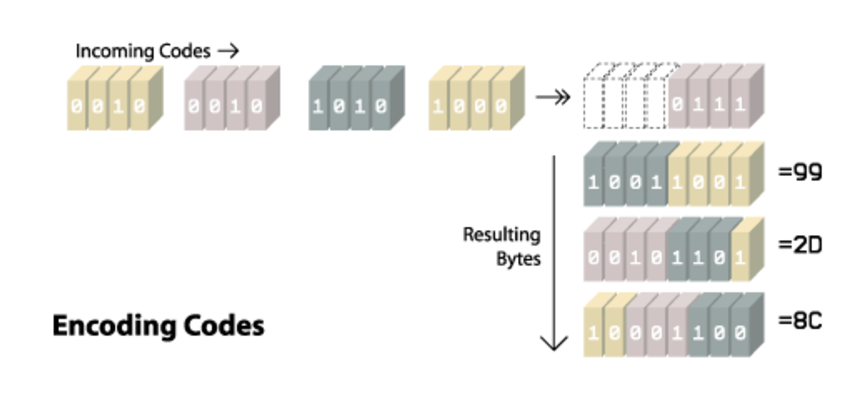
\includegraphics[width=0.6\linewidth]{imagenes/lzw_encoding_codes.eps}
		\end{figure}

	\end{frame}

%----------------------------------------------------------------------------------------

	\begin{frame}
		\frametitle{¿Qué es LZW?}
		La función hash, básicamente, se emplea como método para mapear datos de tamaño o longitud arbitrarios en bloques de un tamaño fijo, de manera que la más mínima diferencia en los datos de entrada de la función genera drásticas diferencias en la salida. Aplicación de esto sería ssh
		\begin{figure}
			\includegraphics[width=0.55\linewidth]{imagenes/Hash.png}
		\end{figure}

	\end{frame}

%----------------------------------------------------------------------------------------

	\begin{frame}
		\frametitle{Compresor LZW}

		\begin{figure}
			\includegraphics[width=0.7\linewidth]{imagenes/compresorpng.png}
		\end{figure}

	\end{frame}
	%----------------------------------------------------------------------------------------
	\begin{frame}
		\frametitle{Análisis de complejidad}
		De acuerdo con el análisis de complejidad, para el peor escenario tenemos
		
		\begin{equation}
			\Theta\left(n^2 \right);\quad O\left(n^2 \right);\quad o\left(n^3 \right);\quad \Omega\left(n \right);\quad\omega\left(n \right)
		\end{equation}
		Para el mejor escenario tenemos:
		\begin{equation}
			\Theta\left(n^0 \right);\quad O\left(n^0 \right);\quad o\left(n \right);\quad \Omega\left(n^{-1} \right);\quad\omega\left(n^{-1} \right)
		\end{equation}

	\end{frame}
%----------------------------------------------------------------------------------------
	\begin{frame}
		\frametitle{Análisis de correctitud}
		Se emplea el invariante de ciclo ''\textit{El índice más el caracter son una nueva entrada, o ya está guardado}''. Se obtienen las siguientes conclusiones para inicialización, mantenimiento y finalización:
		
		\begin{itemize}
			\item \textbf{Inicialización:} Cuando se obtiene el primer valor, como la tabla está inicializada en 0, al aplicar el hash, se va a obtener un nuevo valor, por lo que sería una nueva entrada.			
		\end{itemize}				
		
	\end{frame}
%----------------------------------------------------------------------------------------
	
	\begin{frame}
	\frametitle{Análisis de correctitud}
		\begin{itemize}
			\item \textbf{Mantenimiento:} Si durante el proceso de llenado de la tabla, se da el peor caso que es que la tabla está llena, implicaría que ya existe el hash que estamos analizando, por tanto siempre sería un valor previamente guardado, cumpliéndose el invariante.

			\item \textbf{Terminación:} Dado el último valor, puede darse el peor caso, que como se mencionó antes implicaría que el valor ya está previamente guardado, si fuese un nuevo caracter, simplemente se guardaría en la tabla para ser procesado, para finalmente el final del archivo hiciera el break y terminar la ejecución del programa.
		\end{itemize}			
	
	\end{frame}		

%----------------------------------------------------------------------------------------
	\begin{frame}
		\frametitle{Descompresor LZW}
		
		\begin{figure}
			\includegraphics[width=0.5\linewidth]{imagenes/descompresor.png}
		\end{figure}

	\end{frame}	%----------------------------------------------------------------------------------------
	\begin{frame}
		\frametitle{Análisis de complejidad}
		De acuerdo con el análisis de complejidad, para el peor escenario tenemos
		
		\begin{equation}
			\Theta\left(n^2 \right);\quad O\left(n^2 \right);\quad o\left(n^3 \right);\quad \Omega\left(n \right);\quad\omega\left(n \right)
		\end{equation}
		Para el mejor escenario tenemos:
		\begin{equation}
			\Theta\left(n^0 \right);\quad O\left(n^0 \right);\quad o\left(n \right);\quad \Omega\left(n^{-1} \right);\quad\omega\left(n^{-1} \right)
		\end{equation}

	\end{frame}
%----------------------------------------------------------------------------------------
	\begin{frame}
		\frametitle{Análisis de correctitud}
		Se emplean dos invariantes de ciclo. El primero es ''\textit{El código existe dentro de la tabla hash o es uno nuevo
}''. Se obtienen las siguientes conclusiones para inicialización, mantenimiento y finalización:
		
		\begin{itemize}
			\item \textbf{Inicialización:} para el primer dato, dado que la tabla está en cero, hay que guardarlo, por tanto es un valor nuevo.
		\end{itemize}				
		
	\end{frame}
%----------------------------------------------------------------------------------------
	
	\begin{frame}
	\frametitle{Análisis de correctitud}
		\begin{itemize}
			\item \textbf{Mantenimiento:}  Durante el proceso de llenado de la tabla, si se da una repetición de hash, significa que el código ya está guardado, por tanto ya existe dentro de la tabla hash.


			\item \textbf{Terminación:} Si no hubiesen colisiones, la tabla hash se llena con puros valores nuevos, caso contrario, el último valor choca y haría que ya existiese el valor dentro de la tabla.

		\end{itemize}			
	
	\end{frame}		

%----------------------------------------------------------------------------------------

%----------------------------------------------------------------------------------------
	\begin{frame}
		\frametitle{Análisis de correctitud}
		La segunda invariante es ''\textit{El valor del índice de la tabla hash corresponde a un valor distinto de 0 para la siguiente posición en la tabla y se guarda en el LIFO, o es 0 y se limpia el LIFO}''. Se obtienen las siguientes conclusiones para inicialización, mantenimiento y finalización:
		
		\begin{itemize}
			\item \textbf{Inicialización:} cuando llega el primer código de índice, el valor se guarda en la tabla de hash. Se carga y se analiza, como es el primero existen dos opciones, o es parte de un código nuevo, lo que implicaría que su índice no es cero, por lo que se debe guardar en el LIFO, o que el valor sea un código único, lo que implicaría que su índice es 0 y se pasa directamente al archivo de salida. Sin embargo, dado que la idea original es comprimir un archivo, lo más probable es que sea un código con un índice distinto de 0.

		\end{itemize}				
		
	\end{frame}
%----------------------------------------------------------------------------------------
	
	\begin{frame}
	\frametitle{Análisis de correctitud}
		\begin{itemize}
			\item \textbf{Mantenimiento:}  Cuando ya se vaya llenando la tabla, habrá colisiones que harán que se vaya obteniendo nuevos índices. Si hay un choque en la tabla de hash, esto indicará que el valor ya está en la tabla, por lo que su índice es distinto de cero y pasará a ser guardado en el LIFO. Si fuese el último código de la trama, su índice sería 0 y pasaría a formar parte del documento que se está creando, a su vez que el LIFO va a vaciarse en el orden "último en entrar, primero en salir". Por tanto se cumple el invariante.



			\item \textbf{Terminación:} Para el último valor del archivo, este siempre será único, pues fue el primer valor que se guardó en la tabla para la compresión, por lo que su índice siempre será 0, por lo que se cumple el invariante también.


		\end{itemize}			
	
	\end{frame}		

%----------------------------------------------------------------------------------------

	
%\begin{frame}
%\frametitle{Blocks of Highlighted Text}
%\begin{block}{Block 1}
%Lorem ipsum dolor sit amet, consectetur adipiscing elit. Integer lectus nisl, ultricies in feugiat rutrum, porttitor sit amet augue. Aliquam ut tortor mauris. Sed volutpat ante purus, quis accumsan dolor.
%\end{block}

%\begin{block}{Block 2}
%Pellentesque sed tellus purus. Class aptent taciti sociosqu ad litora torquent per conubia nostra, per inceptos himenaeos. Vestibulum quis magna at risus dictum tempor eu vitae velit.
%\end{block}

%\begin{block}{Block 3}
%Suspendisse tincidunt sagittis gravida. Curabitur condimentum, enim sed venenatis rutrum, ipsum neque consectetur orci, sed blandit justo nisi ac lacus.
%\end{block}
%\end{frame}

%------------------------------------------------

%\begin{frame}
%\frametitle{Multiple Columns}
%\begin{columns}[c] % The "c" option specifies centered vertical alignment while the "t" option is used for top vertical alignment

%\column{.45\textwidth} % Left column and width
%\textbf{Heading}
%\begin{enumerate}
%\item Statement
%\item Explanation
%\item Example
%\end{enumerate}

%\column{.5\textwidth} % Right column and width
%Lorem ipsum dolor sit amet, consectetur adipiscing elit. Integer lectus nisl, ultricies in feugiat rutrum, porttitor sit amet augue. Aliquam ut tortor mauris. Sed volutpat ante purus, quis accumsan dolor.

%\end{columns}
%\end{frame}

%------------------------------------------------
%\section{Second Section}
%------------------------------------------------

%\begin{frame}
%\frametitle{Table}
%\begin{table}
%\begin{tabular}{l l l}
%\toprule
%\textbf{Treatments} & \textbf{Response 1} & \textbf{Response 2}\\
%\midrule
%Treatment 1 & 0.0003262 & 0.562 \\
%Treatment 2 & 0.0015681 & 0.910 \\
%Treatment 3 & 0.0009271 & 0.296 \\
%\bottomrule
%\end{tabular}
%\caption{Table caption}
%\end{table}
%\end{frame}

%------------------------------------------------

%\begin{frame}
%\frametitle{Theorem}
%\begin{theorem}[Mass--energy equivalence]
%$E = mc^2$
%\end{theorem}
%\end{frame}

%------------------------------------------------

%\begin{frame}[fragile] % Need to use the fragile option when verbatim is used in the slide
%\frametitle{Verbatim}
%\begin{example}[Theorem Slide Code]
%\begin{verbatim}
%\begin{frame}
%\frametitle{Theorem}
%\begin{theorem}[Mass--energy equivalence]
%$E = mc^2$
%\end{theorem}
%\end{frame}\end{verbatim}
%\end{example}
%\end{frame}

%------------------------------------------------

%\begin{frame}
%\frametitle{Figure}
%Uncomment the code on this slide to include your own image from the same directory as the template .TeX file.
%\begin{figure}
%\includegraphics[width=0.8\linewidth]{test}
%\end{figure}
%\end{frame}

%------------------------------------------------

%\begin{frame}[fragile] % Need to use the fragile option when verbatim is used in the slide
%\frametitle{Citation}
%An example of the \verb|\cite| command to cite within the presentation:\\~

%This statement requires citation \cite{p1}.
%\end{frame}

%------------------------------------------------

%\begin{frame}
%\frametitle{References}
%\footnotesize{
%\begin{thebibliography}{99} % Beamer does not support BibTeX so references must be inserted manually as below
%\bibitem[Smith, 2012]{p1} John Smith (2012)
%\newblock Title of the publication
%\newblock \emph{Journal Name} 12(3), 45 -- 678.
%\end{thebibliography}
%}
%\end{frame}

%------------------------------------------------
	\begin{frame}
		\Huge{\centerline{Tiempo para una demostración}}
	\end{frame}
%----------------------------------------------------------------------------------------
	\begin{frame}
		\Huge{\centerline{Gracias por su atención}}
	\end{frame}
%----------------------------------------------------------------------------------------

\end{document} 
